\topskip0pt
\vspace*{\fill}
\begin{center}
    \textit{END OF MASTER}\thispagestyle{empty}
\end{center}
\vspace*{\fill}
%

\chapter{Old Document}
%\begin{preprompt}
%Sketches your basic plan for the system that you will build. If the system is partially built by the midterm delivery deadline, then explain what you have so far along with what you plan to add. In general, the reader should get a good impression of the structure of the complete system that you will eventually deliver for your master's thesis.
%\end{preprompt}


All object detection systems require the same basic units: a model, data loader, evaluator, and data logger.
Figure~\ref{fig:sys} gives an overview of the system with some of the components broken down further.
Some parts of the system have been prototyped at this stage, while others only have basic functionality.
We will go through the components separately in the next sections

\begin{figure}[htb]
  \centering
  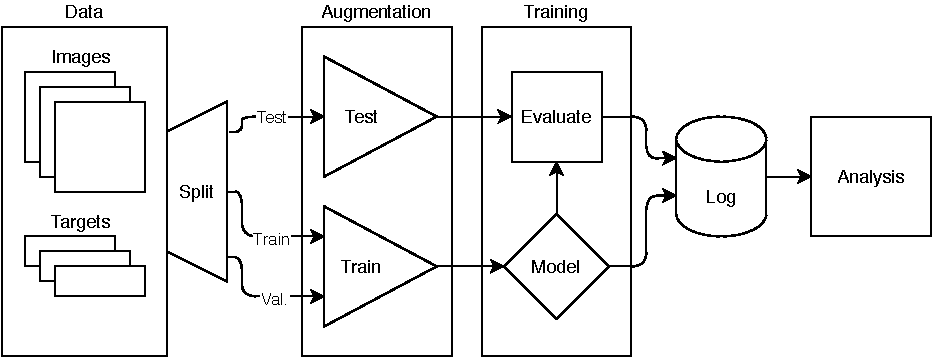
\includegraphics[width=0.7\textwidth]{figs/system.pdf}
  \caption[System overview]{Overview of the basic system components and their interactions.}\label{fig:sys}
\end{figure}

The data loader is responsible for fetching the image files from disk, transforming them to the proper format, and augmenting them.
This system has been developed and is functional.
More types of augmentations can and will be added in the next stage of the project.
The output of the data loader is batches of augmented images and the corresponding labelled bounding boxes.

A prototype of the SSD model has been developed.
The implementation is based on the source code released by the authors.
The main improvements that remain relate to the structure of the system to make it suitable for modification.
It should require no coding to change the backbone model, activation function, batch norm and default box scaling.

The evaluation system has not been developed, only a basic module for visualizing the output of the model.
A completed model would run the model over the testing data and measure the precision, recall, and other relevant performance measures.


\section*{Technology}
%\begin{preprompt}
%Indicates your competence with the tools (often software packages such as TensorFlow, PyTorch, etc.) that will be the foundation of your thesis code. At this point in time, you should FULLY understand those tools, be able to CLEARLY explain them, and be able to run some prototypes related to your final project goals. For example, if you plan to use TensorFlow to implement a complex Boltzmann Machine on a complex problem, you should be able to hack up a prototype of a SIMPLE Boltzmann Machine on a SIMPLE task at this point.
%\end{preprompt}

The software implementation for this project is written in Python using the PyTorch library~\parencite{NEURIPS2019_9015} for all computational tasks.
PyTorch includes sub packages for handling the entire deep learning pipeline, i.e.~all sections shown in Figure~\ref{fig:sys}.
PyTorch is a relatively new framework but has quickly become one of the most popular tools, especially in research.
The two main reasons for this are the \textit{pythonic} API design and its \textit{dynamic computational graph}.
The API is designed from the bottom up to integrate into the already established python data science ecosystem as well as to follow the common design goals of being clear and consistent.
One of the most complicated aspects of training neural networks is computing the derivatives for all the parameters.
All modern frameworks perform automatic differentiation using a \textit{computational graph} which tracks the computations applied to the tensors through the forward pass.
The gradients are then calculated by following this graph from the Loss and back through to the input.
Most frameworks operate using a \textit{static} graph which is calculated and stored before the training can start.
PyTorch instead uses a \textit{dynamic} approach where the computational graph is calculated at runtime with each forward pass, allowing the model to potentially change structure.
This property is not something this implementation drawn any obvious benefits, but it results in a very modular design patters, making it relatively straight forward to implement any model using the library as intended.  


\section*{Data}
The dataset used for training the prototype is provided by~\cite{gallardo_caballero_precise_2019}.
The dataset contains a total of 390 images and 2037 ground truth boxes.
Class labels are omitted from the dataset so the model could only be trained to predict the binary prediction \textit{\{Pollen, Background\}}.
The images contain RGB with the same dimensions, \( 640\by 512 \) pixels.

\begin{figure}[htbp]
  \centering
  \begin{subfigure}[b]{0.4\textwidth}
    \centering
    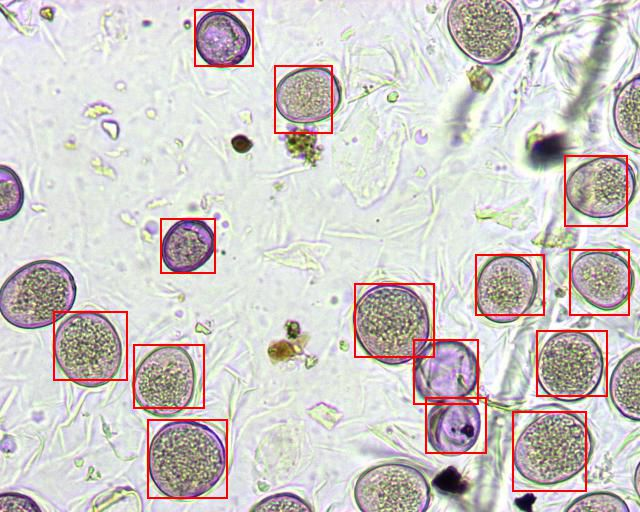
\includegraphics[width=\textwidth]{figs/ex_04}
    \vspace*{0.02\textwidth}
  \end{subfigure}%
  \hspace*{0.04\textwidth}
  \begin{subfigure}[b]{0.4\textwidth}
    \centering
    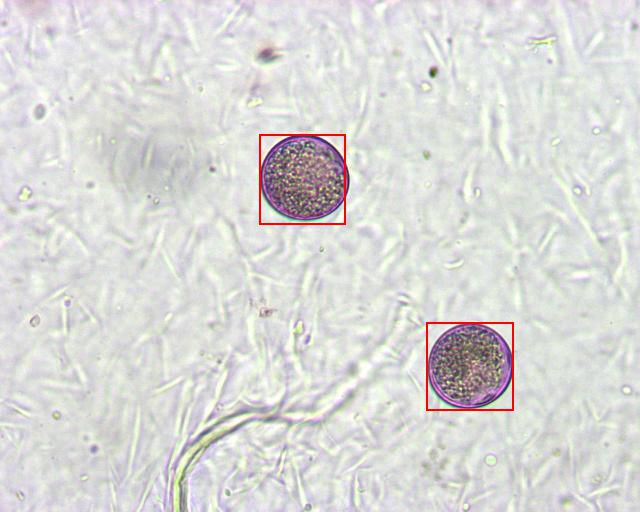
\includegraphics[width=\textwidth]{figs/ex_03}
    \vspace*{0.02\textwidth}
  \end{subfigure}

  \begin{subfigure}[t]{0.4\textwidth}
    \centering
    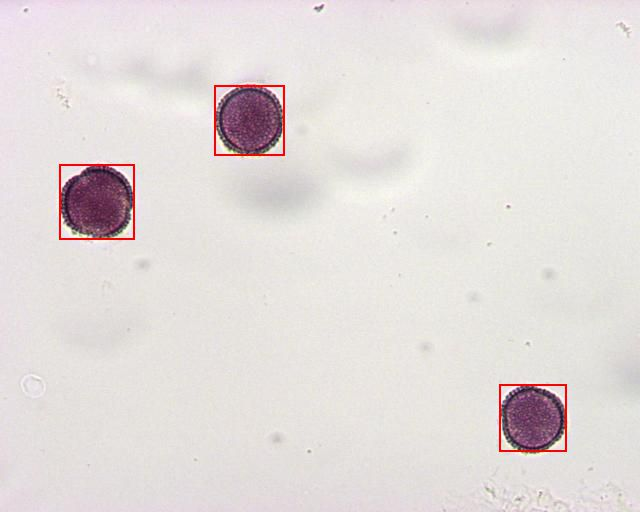
\includegraphics[width=\textwidth]{figs/ex_02}
  \end{subfigure}%
  \hspace*{0.04\textwidth}
  \begin{subfigure}[t]{0.4\textwidth}
    \centering
    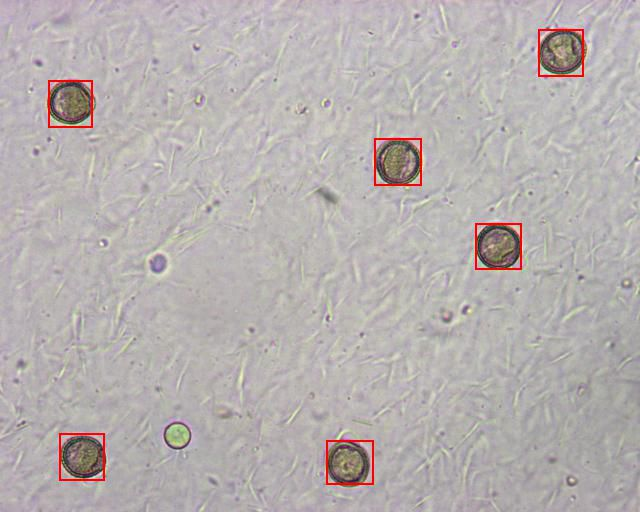
\includegraphics[width=\textwidth]{figs/ex_01}
  \end{subfigure}
  \caption[Examples from dataset]{
    Examples from the training data.
    The images vary in background and lighting conditions.
    Ground truths in \textcolor{red}{red}.}\label{fig:training}
\end{figure}


\subsection*{Augmentations}
The augmentations were inspired by the original SSD implementation.
Augmentations are vitally important with a data set this small.
The following procedure was used for the training procedure:
\begin{enumerate}
  \item Crop to 300px square containing \( \geq 1 \) ground truth box.
  \item With an independently calculated 50\% chance do any/all of the following:
  \begin{enumerate}
  \item Horizontal flip.
  \item Vertical flip.
  \item Shuffle channels.
  \item Color shift (brightness, contrast, and saturation).
  \end{enumerate}
\end{enumerate}

With this procedure there are 16 possible combinations of augmentations that could be applied to each image, significantly increasing the apparent size of the dataset.

\section*{Preliminary Results}
The results of training the prototype model show evidence of learning but have also revealed issues that make it very hard to measure the performance.
Examples of the predictions are given in Figure~\ref{fig:pred}.
Most of the predicted boxes are concentrated around pollen grains, but because they are too small, none of them can be classified as correct.
This result is consistently found across the test set and indicates an error somewhere in the implementation.
The cause of the issue has not been found as of writing but is most likely due to an error in either the loss calculation.

\begin{figure}[htbp]
  \centering
  \begin{subfigure}[t]{0.4\textwidth}
    \centering
    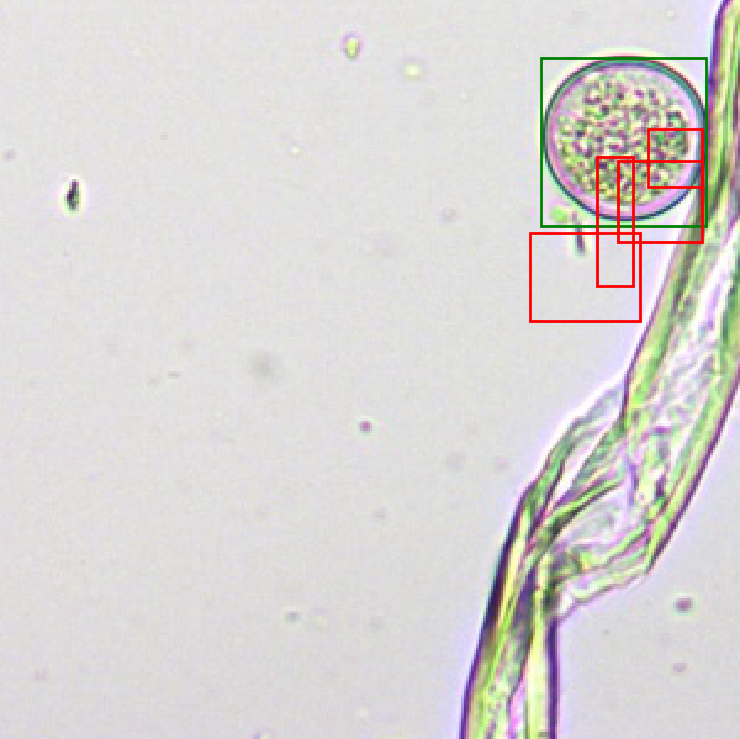
\includegraphics[width=\textwidth]{figs/infer_01}
  \end{subfigure}%
  \hspace*{0.04\textwidth}
  \begin{subfigure}[t]{0.4\textwidth}
    \centering
    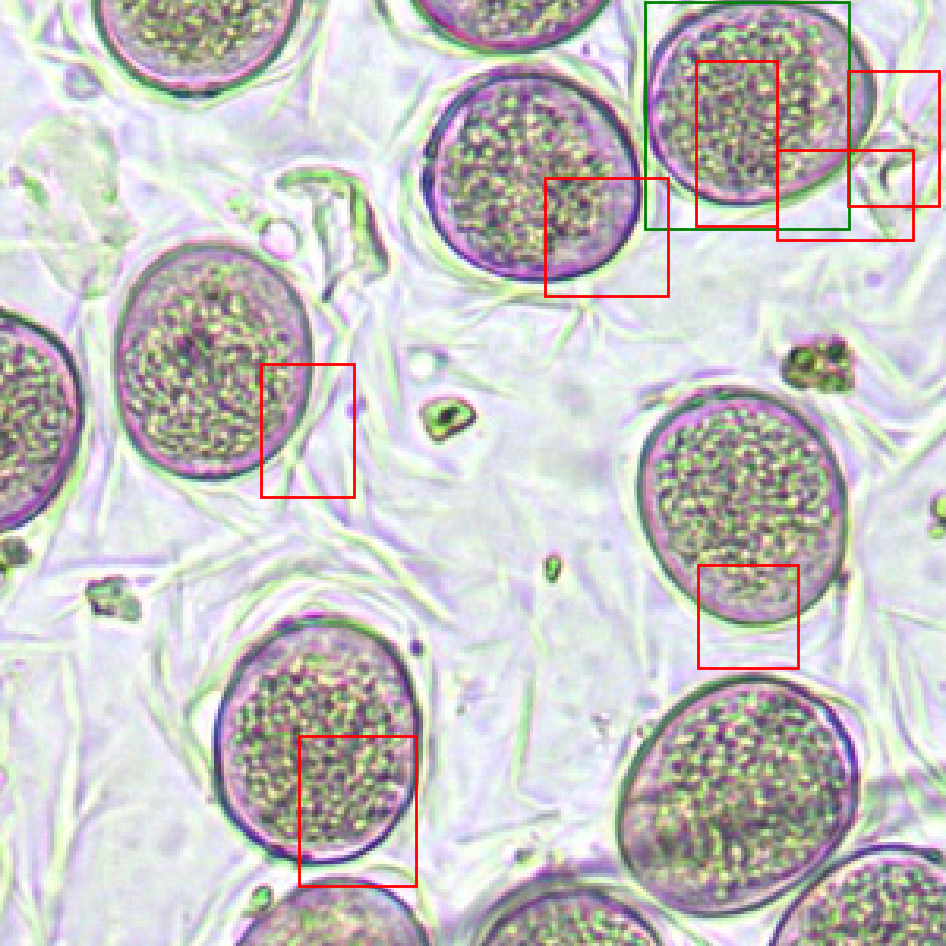
\includegraphics[width=\textwidth]{figs/infer_02}
  \end{subfigure}
  \caption[Example predictions]{Example predictions made by the trained model.
The model shows clear indications of learning, but the predictions seem to be consistently too small to be considered correct.
Predictions in \textcolor{red}{red}, ground truths in \textcolor{nicegreen}{green}.}\label{fig:pred}
\end{figure}

The preliminary results are promising, but also show that there are improvements that need to be made before any experiments can be run.
In particular, the training problems must be solved and a dataset with labelled classes must be acquired.
We will address these issues further in the next section, as we detail the plans for the remainder of this project.

\section*{Future Plans}
%\begin{preprompt}
%Lays out your plans for the main tests that you will perform with your model, along with possible model variants or extensions that you might want to investigate (given enough time). It should also sketch a basic timeline for your writing and coding activities during the upcoming 5--6 months of your master work.
%\end{preprompt}

With the completion of this thesis project, we have established how our system fits in with the surrounding research, and in what ways our work could add to this field.
However, before we are able to produce any results, there are three major checkpoints that need to be completed.
Firstly, we must finalize the model, meaning it must be able to run experiments, and validate the results.
The learning issues we have discovered also need to be addressed, such that the baseline model actually converges to an acceptable solution.
Secondly, we must prepare a new dataset which has both bounding boxes and class labels.
Lastly, we must design the exact specifications of each experiment.


\section*{Model}
The overview of the development, as described in Section~\textbf{??} provides the outline for what remains to be done in the next stage of the project regarding the system.
We estimate that the majority of the total time needed to develop the system has been expended, and that the time remaining to finalize is in the order of weeks.

When completed the system will take in a labelled train/val dataset and run a training session with either early stopping or for a set number of epochs, then it will run evaluation and the validation set, calculating precision, recall.

Given that the model we are using is many years old at this point, the baseline we establish will most like utilize newer features, such as batch normalization.
Establishing the baseline model will therefore also offer a chance to compare different techniques that have not been tested in this domain before.

\section*{Data}
The process of acquiring a new dataset has already begun, but a thorough discussion on the process is left to the next stage of the project.
The data has been provided by The Norwegian Asthma and Allergy Association (NAAF) and consists of slides of pollen acquired from pollen monitoring stations. 

Pollen is collected with traps where air is continually sucked though a small slit and over an adhesive strip.
The strip is moved across the slit, exposing different sections throughout the day.
Pollen grains and other air born particulates adhere to the strip, which is then analyzed under a microscope.
This produces an estimate for the density of different pollen types, measured in particles per cubic meter, throughout the season. 

The dataset used three microscope slides which were photographed using LM imaging.
The total amount of images and labels is unknown as of writing.
Due to the varying flowering seasons of the various species that are analyzed, only 2--3 different classes of pollen are observed on any one slide, the total number of classes in the dataset most likely be in the range 3--5.
This dataset is also easily extended, given the fact that historic data from multiple collection stations over multiple seasons exist.
If the developed system were to produce good results, this process could also be accelerated in future iterations.

After the data is collected and labelled it must be partitioned into a training set and testing set.
This process should be semi random, but it is important to balance the datasets in such a way that the distribution of classes is equal.

\section*{Experiments}
There are three main experiments that must be designed and executed.
Firstly, various configurations of models must be tested to establish a well performing baseline model.
Secondly the model must be simplified in different ways so that the impact of the changes can be measured.
Third we must incorporate multifocal data into either the training or inference operation and measure the impact.

\subsection*{Baseline}
As mentioned, newer techniques have been used in other object detection frameworks that have been published after SSD\@.
These relate to e.g.\ normalization, activation functions, parameter initialization, and bounding box regression parameters.
Of these most are available in PyTorch and are almost trivial to add to the basic SSD\@.
Training times for the prototype model have been on the order of hours, so testing a variety of techniques.
Tuning the hyper parameters for the optimizer also falls under this category of experiments.

\subsection*{Simplification}
There are three main ways to simplify the SSD model.
Firstly, we can remove feature layers from the auxiliary structure, thereby limiting the range of scales of the default boxes.
This can by visually explained as removing blocks from Figure~\ref{fig:model}.
Secondly, we can reduce the number of default boxes per feature map.
The original model uses 6 default boxes per anchor point with different aspect ratios, any number below this could by testes.
Thirdly, we can use a smaller backbone, meaning one with fewer parameters.

This thesis has attempted to determine how a CNN object detection can be used to further the progress toward creating a system for automatic pollen counting.
We have uncovered opportunities for unique contributions to the existing knowledge-base that we hope a fully developed system may be able to deliver.
By the end of the project, we hope to demonstrate that a computationally inexpensive model may be capable of performing the task of counting and classifying pollen grains.
